\documentclass[dvipdfmx,autodetect-engine,titlepage]{jsarticle}
\usepackage[dvipdfm]{graphicx}
\usepackage{ascmac}
\usepackage{fancybox}
\usepackage{listings}
\usepackage{plistings}
\usepackage{itembkbx}
\usepackage{amsmath}
\usepackage{svg}
\usepackage{url}
\usepackage{graphics}
\usepackage{listings,jvlisting}

\textheight=23cm
\renewcommand{\figurename}{図}
\renewcommand{\tablename}{表}
\newenvironment{code}
{\vspace{0.5zw}\VerbatimEnvironment  
\begin{screen} 
\baselineskip=1.0\normalbaselineskip
 \begin{Verbatim}}
{\end{Verbatim}
\baselineskip=\normalbaselineskip
 \end{screen}\vspace{0.5zw}} 

\title{情報理工学部 SNコース 2回\\
材料と化学\\
第二回レポート}
\author{2600200443-6\\Yamashita Kyohei\\山下 恭平}
\date{Dec 7 2021}

\begin{document}

\maketitle

\section{概要}
二次電池について調べる。\\
二次電池とは一次電池と異なり、充電を行うことで繰り返し使用可能な電池のこと
である。

\section{開発の歴史}
初めて開発された二次電池は、一次電池が開発されてから約60年後、1859年にフラ
ンス人科学者のガストン・プランテによって開発された鉛蓄電池である。それから40
年後にはスウェーデン人科学者のユングナーによってニッケルカドミウム電池が、1900
年にはエジソンによりニッケル・鉄電池が、1964年には ニッケルカドミウム電池、
1990年にはニッケル水素電池、そして1991年にはリチウムイオン電池が開発されてい
きました。初めて開発された二次電池である鉛蓄電池は現在でも使用されており、160
年以上の歴史を持っています。

\section{組成・構造・特性・性質}

  \subsection{鉛蓄電池}
  鉛蓄電池は正極には酸化鉛、負極には鉛が、電解液には希硫酸が使用されている。
  基本的な構造として、電解液の中に二種類の電極を入れることで起きる化学反応
  により硫酸イオンが移動することで、充電、放電を行う。材料が安価で比較的高
  電圧を取り出せるが、大きく重たいという特徴を持つ。主に自動車のバッテリー
  などに使用されている。
  \begin{figure}[h]
    \begin{minipage}[b]{0.45\linewidth}
    \begin{center}
      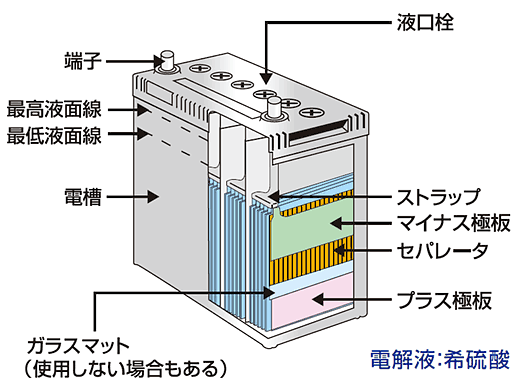
\includegraphics[keepaspectratio,scale=0.3]{SodaPDF-converted-pic1.png}
      \end{center}
      \caption{鉛蓄電池構造 *1}
    \end{minipage}
    \begin{minipage}[b]{0.45\linewidth}
    \begin{center}
      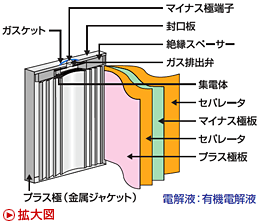
\includegraphics[keepaspectratio,scale=0.5]{SodaPDF-converted-pic2.png}
      \end{center}
      \caption{リチウムイオン電池構造 *2}
    \end{minipage}
  \end{figure}

  \subsection{リチウムイオン電池}
  リチウムイオン電池は主に,正極にはコバルト酸リチウム、負極にはリチウム貯蔵炭素が、
  電解液には非水系の有機溶解液が使用されている。基本的な構造として、電解液、
  電極、セパレータで構成され、リチウムイオンの動きによって電気の放電、充電を
  行なっている。現在では二次電池の半分以上がリチウムイオン電池であり、軽量、
  小型化、大容量、高電圧などといったかなり高い性能を持つが、価格が高く、安全
  性などにも若干の問題を抱える。スマートフォン、コンピュータ、電気自動車などの
  バッテリーに使用されている。


  \subsection{ニッケル水素電池}
  この電池の正極にはニッケルの酸化物であるオキシ水酸化ニッケル,負極には水素
  吸蔵合金,電解液には水酸化カリウムのアルカリ水溶液が使われている。基本的な
  構造として、電解液、電極、セパレータで構成され、化学反応で生まれる電子の
  動きによって、充電、放電を行う。ニッケルカドミウム電池と異なり、有害物質を
  含んでおらず、電池容量も大きいことから置き換えが進んでいる、温度によって
  性能差が出てしまう。充電し繰り返し使用できる乾電池や電気自動車のバッテリー
  などに使用されている。
  \begin{figure}[h]
    \centering
    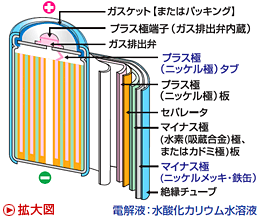
\includegraphics[scale=0.4]{SodaPDF-converted-pic3.png}
    \caption{ニッケル水素電池構造  *3}
  \end{figure}

  \section{今後の電池と発電}
  現代社会、EV化が進むこの世の中においてバッテリーの需要はどんどん上がっていく
  と考えられる。すでにTeslaは電気自動車のみの販売で世界に名を轟かしており、
  多くの日本の自動車メーカーも電気自動車産業に移行していくことが発表されている。
  電気自動車で私が最も気になっていることは航続距離がガソリン車に比べて短いこと
  である。当然私だけではなく、多くのメーカーがその問題について研究を続けているので
  今後さらに、バッテリーの容量は増えていくと考えられる。電池の進化と同時に
  発電の方法についても大きな進歩が必要だと私は考えている。電気はクリーンエネ
  ルギーであると言われれば確かにそうだと感じてしまうが、その電気を発電するために
  多くの二酸化炭素が排出されている事実があるかぎり、クリーンエネルギーとは呼べないと
  私は考えている、今後、電気自動車の割合が増え、発電量も増えることが予想されるが、
  このことが本当に環境に良いのかどうか改めて考え、理解する必要があると私は考えた。

\section{参考文献}

*1,2,3\\
一般社団法人 電池工業会\\
\url{https://www.iae.or.jp/wp/wp-content/uploads/2014/09/2008-1.pdf}\\

エネルギー総合科学研究所\\
\url{https://www.iae.or.jp/wp/wp-content/uploads/2014/09/2008-1.pdf}\\

INFUSE バッテリー再生事業\\
\url{https://www.infuse-net.com/articles/articles005.html}\\


\end{document}

